\documentclass[twoside,10pt]{article}
\usepackage{amsmath,amsfonts,amsthm,fullpage,amssymb}
%\usepackage{mymath}
\usepackage{algorithm}
\usepackage{algorithmic}
\usepackage{graphicx}
\usepackage{url}


\begin{document}


\title{ISYE 6740 Homework 5\\ 
\small Total 100 points.}
%\author{Yao Xie}
%\date{Deadline: Feb. 13, Sat., 11:55pm}
\date{}
\maketitle



As usual, please submit a report with sufficient explanation of your answers to each the questions, together with your code, in a zip folder.

%----------------------------------------------------------------------------------

\begin{enumerate}

\item {\bf Comparing SVM and simple neural networks.} (50 points)

This question is to implement and compare {\bf SVM and simple neural networks} for the same datasets we tried for the last homework. We suggest to use \textsf{Scikit-learn}, which is a commonly-used and powerful \textsf{Python} library with various machine learning tools. But you can also use other similar libraries in other programming languages of your choice to perform the tasks. 

You may use a neural networks function \textsf{sklearn.neural\_network} with \textsf{hidden\_layer\_sizes=(5, 2)}. Tune the step size so you have reasonable results. You may use \textsf{svc} and tune the penalty term $C$ to get reasonable results. 

\textbf{Part One (Divorce classification/prediction).} (30 points) 

We will compare using the same dataset as the last homework, which is about participants who completed the personal information form and a divorce predictors scale. 

The data is a modified version of the publicly available at \url{https://archive.ics.uci.edu/ml/datasets/Divorce+Predictors+data+set} (by injecting noise so you will not replicate the results on uci website). There are 170 participants and 54 attributes (or predictor variables) that are all real-valued. The dataset \textbf{q3.csv}. The last column of the CSV file is label $y$ (1 means ``divorce'', 0 means ``no divorce''). Each column is for one feature (predictor variable), and each row is a sample (participant). A detailed explanation for each feature (predictor variable) can be found at the website link above. Our goal is to build a classifier using training data, such that given a test sample, we can classify (or essentially predict) whether its label is 0 (``no divorce'') or 1 (``divorce''). 

Build two classifiers using SVM and a simple neural networks. First random shuffle the data set. Then use the first $80\%$ data for training and the remaining $20\%$ for testing. If you use \textsf{scikit-learn} you can use \textsf{train\_test\_split} to split the dataset. 

\begin{enumerate}

	\item (15 points) Report testing accuracy for each of the two classifiers.  Comment on their performance: which performs better and make a guess why it performs better in this setting. 
	\item (15 points) Use the first two features to train two new classifiers. Plot the data points and decision boundary of each classifier. Comment on the difference between the decision boundary for the two classifiers. Please clearly represent the data points with different labels using different colors.
\end{enumerate}

\textbf{Part Two (Handwritten digits classification).} (20 points) Repeat the above part (a) using the \textbf{MNIST Data} in our \textbf{Homework 3}. Here, give ``digit'' 6 label $y = 1$, and give ``digit'' 2 label $y = 0$. All the pixels in each image will be the feature (predictor variables) for that sample (i.e., image). Our goal is to build classifiers such that given a new testing sample, we can tell it is a 2 or a 6. Using the first $80\%$ of the samples for training and remaining $20\%$ for testing. Report the classification accuracy on testing data, for each of the two classifiers. Comment on their performance: which performs better and make a guess why they perform better in this setting. 

\clearpage
\item  {\bf AdaBoost.} (50 points)

Consider the following dataset, plotting in Figure 1. The first two coordinates represent the value of two features, and the last coordinate is the binary label of the data.
\begin{equation*}
\begin{split}
&X_1 = (-1, 0, +), X_2 = (-0.5, 0.5, +), X_3 = (0, 1, -), X_4 = (0.5, 1, -), \\
&X_5 = (1, 0, +), X_6 = (1, -1, +), X_7 = (0, -1, -), X_8 = (0, 0, -).
\end{split}
\end{equation*}

In this problem, you will run through $T = 3$ iterations of AdaBoost with decision stumps (axis-aligned half planes) as weak learners.

\begin{enumerate}
\item (30 points) For each iteration $t = 1, 2, 3$, compute $\epsilon_t$, $\alpha_t$, $Z_t$, $D_t$ by hand (i.e., show all the calculation steps) and draw the decision stumps on Figure 1. Recall that $Z_t$ is the normalization factor to ensure that the weights $D_t$ sum to one. ({\it Hint: At each iteration, you may specify  any reasonable decision rule $h_t$ as you would like.})

\item (20 points) What is the training error of AdaBoost? Give a one-sentence reason for why AdaBoost outperforms a single decision stump.
\end{enumerate}

\clearpage

\begin{figure}
\begin{center}
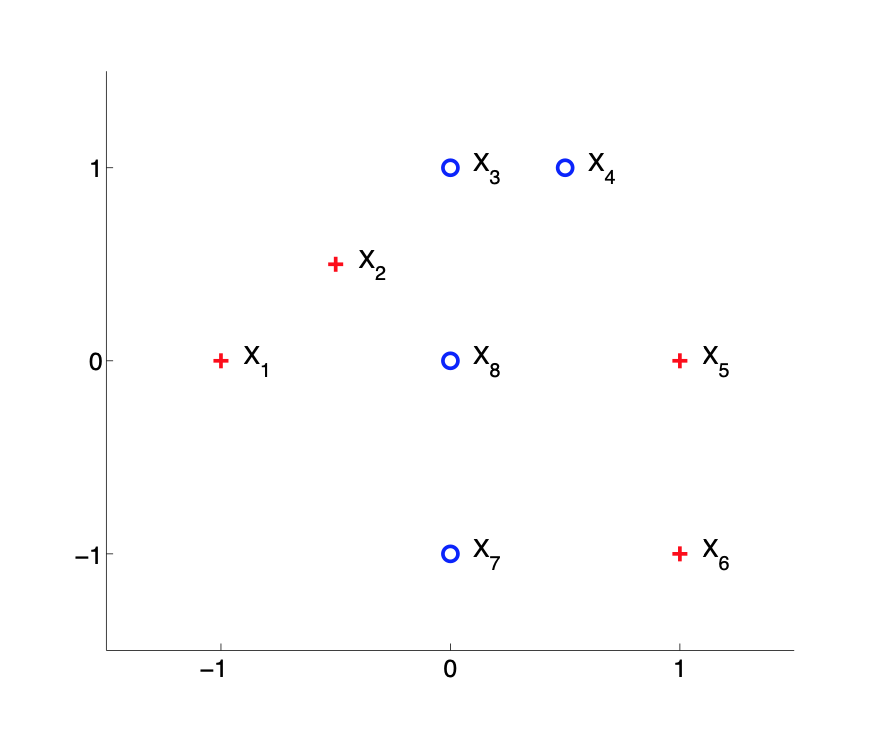
\includegraphics[width = 1\textwidth]{hw}
\end{center}
\caption{ A small dataset, for binary classification with AdaBoost.}
\end{figure}
\end{enumerate}

\begin{table}
\begin{center}
\caption{Values of AdaBoost parameters at each timestep.}
\vspace{0.1in}
\begin{tabular}{|c|c|c|c|c|c|c|c|c|c|c|c|}\hline
t & $\epsilon_t$ & $\alpha_t$ & $Z_t$ & $D_t(1)$ & $D_t(2)$ & $D_t(3)$ & $D_t(4)$ & $D_t(5)$ & $D_t(6)$ & $D_t(7)$ & $D_t(8)$ \\\hline
1 & & & & & & & & & & & \\
2 & & & & & & & & & & &\\
3 & & & & & & & & & & & \\\hline
\end{tabular}
\end{center}
\end{table}



\end{document}
